a)
Jeg udfører samtlige forskellige regressioner, og det viser sig at en kvadratisk regression passer bedst med en $R^2$-grad på 98.8776 med funktionsforskriften $f(x)=0.00057927x^2+0.44741x+29.275$
\begin{figure}[H]
    \centering
    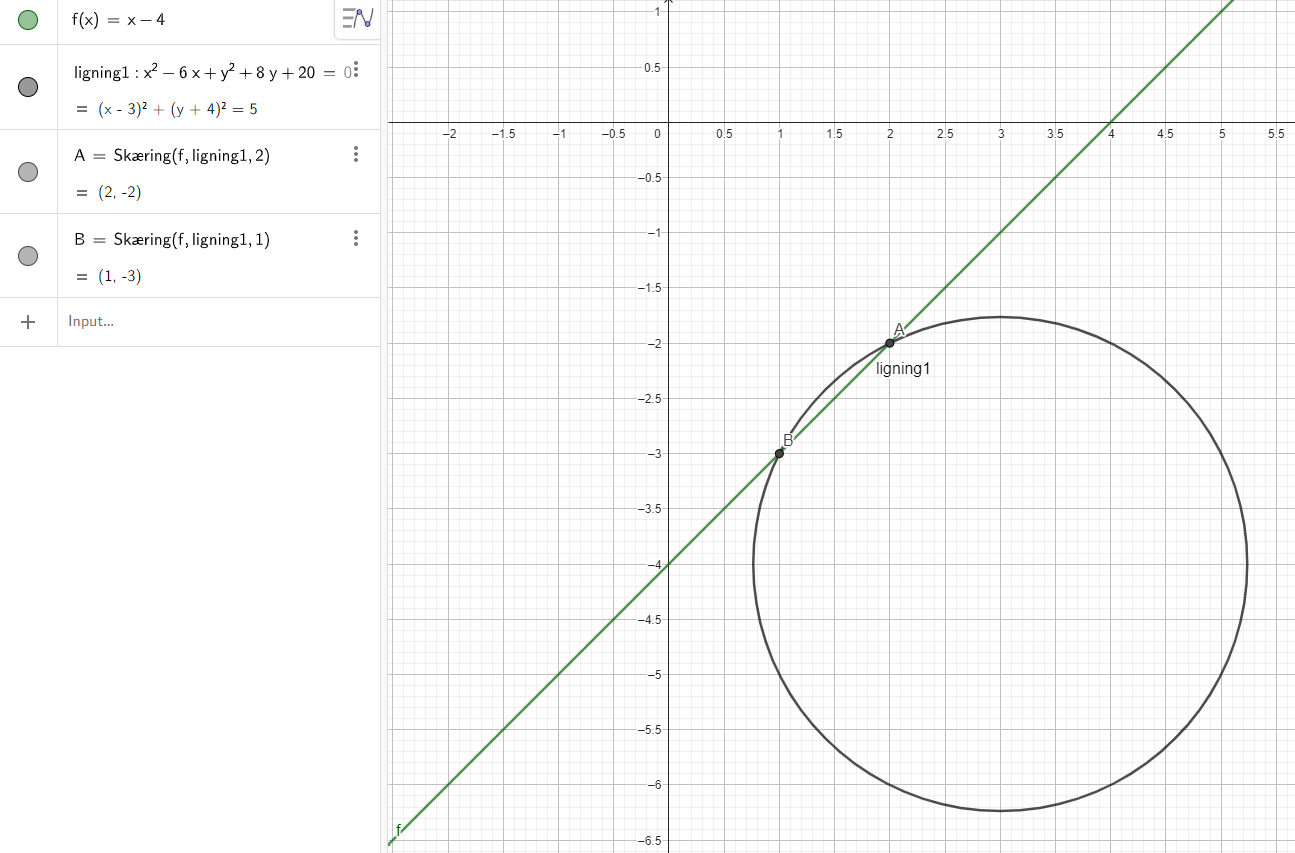
\includegraphics[width=1\linewidth]{Billeder/image.png}
\end{figure}

\begin{figure}[H]
    \centering
    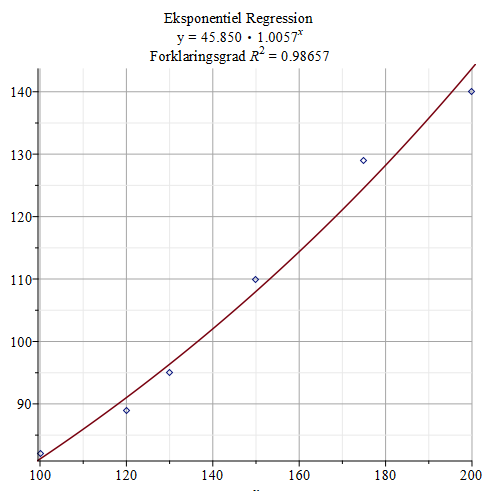
\includegraphics[width=1\linewidth]{Billeder/image2.png}
\end{figure}

\begin{figure}[H]
    \centering
    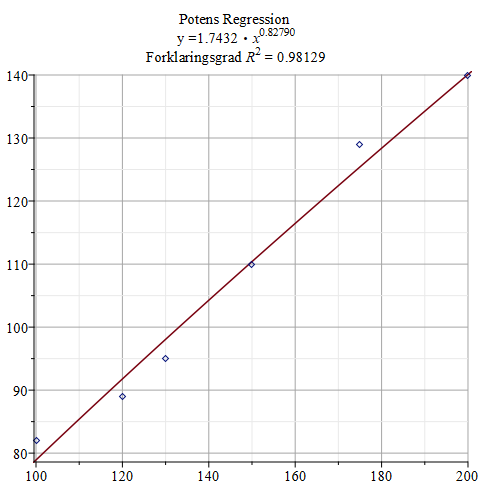
\includegraphics[width=1\linewidth]{Billeder/3.png}
\end{figure}

\begin{figure}[H]
    \centering
    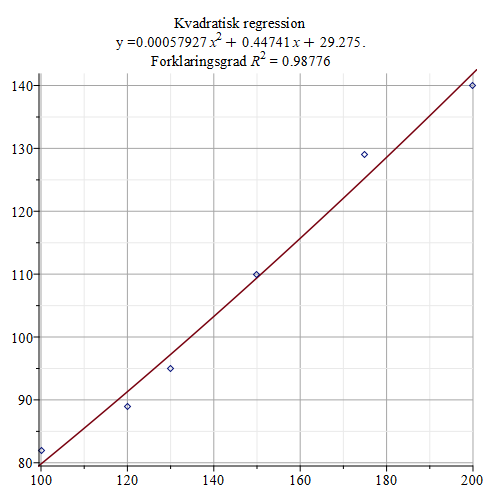
\includegraphics[width=1\linewidth]{Billeder/4.png}
\end{figure}

b)
Jeg kan bruge funktionsforskriften og isolere x:
$$f(x)=0.00057927\cdot x^2 + 0.44741x + 29.275\Longleftrightarrow 121 = 0.00057927x^2 + 0.44741x + 29.275$$
Her bruger jeg Maple til at isolere x:
$$x = 168.3282343 \quad \cap \quad -940.6969052$$
I denne opgave giver det ikke mening af en mand skulle kune have en arbejdsbelastning, der er negativ, derfor må svaret være ca. $168.32$.\newpage